\section{ГРАФИЧЕСКИЙ ИНТЕРФЕЙС ПОЛЬЗОВАТЕЛЯ}
Графический интерфейс был разработан с помощью библиотеки <<PySide6>> \cite{pyside}. 
Были созданы следущие виджеты:
\begin{enumerate}
    \item виджет для визуализации графа;
    \item виджет для создания информации о графе;
    \item виджеты для создания графа, согласно каждой
        из моделей генерации случайного графа;
    \item виджеты для визуализации поиска в глубину и ширину;
    \item виджет для создания графа и подсветки в нем мостов;
\end{enumerate}

Рассмотрим примеры работы данного приложения
\begin{figure}[H] 
    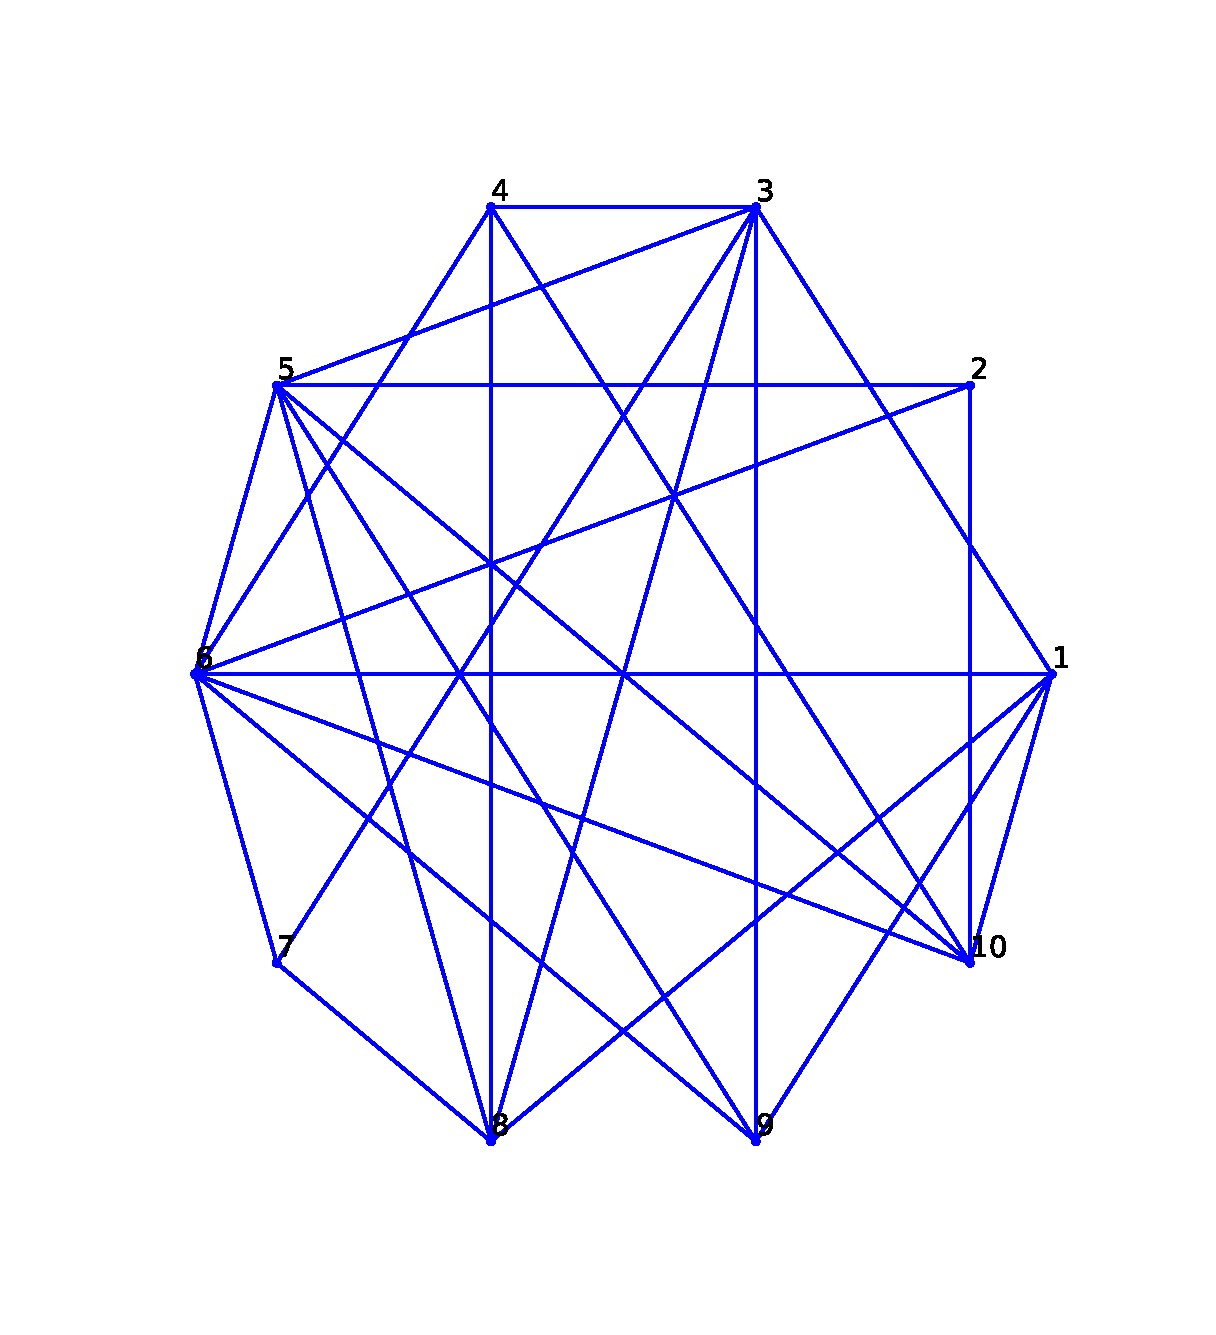
\includegraphics[scale=0.5]{g1.png}
    \caption{Граф с подсвеченным мостом}
    \label{gui_1}
\end{figure} 
На рисунке \ref{gui_1} приведено основное окно графического приложения.
\begin{figure}[H] 
    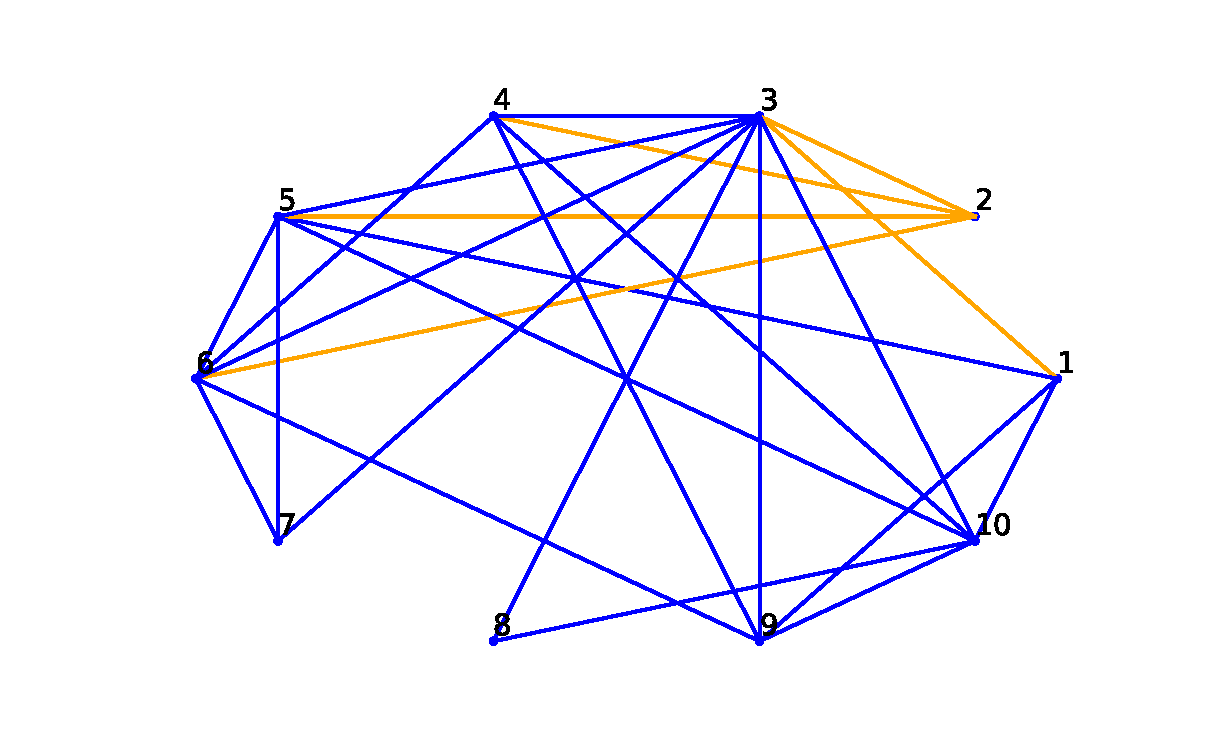
\includegraphics[scale=0.5]{g2.png} 
    \caption{Диаграмма распределения степеней вершин графа.}
    \label{gui_2}
\end{figure} 
На рисунке \ref{gui_2} изобржена диаграмма распределения
степеней графа, приведенного на рисунке \ref{gui_1}.
\begin{figure}[H] 
    \includegraphics[scale=0.5]{g3.png} 
    \caption{Характеристики графа.}
    \label{gui_3}
\end{figure} 
На риcунке \ref{gui_3} приведены характеристики
графа, привденного на рисунке \ref{gui_1}.

